\documentclass[11pt]{article}
\usepackage{graphicx}
\usepackage{hyperref}
\usepackage{natbib}
\usepackage{setspace}

\setlength{\textwidth}{6.5in}
\setlength{\headheight}{0in}
\setlength{\textheight}{8.0in}
\setlength{\hoffset}{0in}
\setlength{\voffset}{0in}
\setlength{\oddsidemargin}{0in}
\setlength{\evensidemargin}{0in}
\doublespacing

\title{Computational Physics HW3}
  
\author{Siyuan Chen}


\begin{document}

\maketitle

\section*{}
P1: For $f(x)=x(x-1)$, taking derivative analytically, we get $f\prime(x)=x+x-1=2x-1$. Then $f\prime(1)=1$. Computing the derivative equation, we get delta=0.01, derivative=1.010000000000001. This is not the explicit answer since delta is not perfectly zero. We are not getting the tangent at $x=1$ but the slope between $x=1$ and $x=1.01$ instead. Plug in smaller and smaller delta, we observe that the behavior of derivative gets better first as approaching to the tangent line, but then get worse when $\delta=10^{-14}$ the order difference between $x$ and $\delta$ is of 14. This is when the round-off error starts to dominate.


\section*{}

\begin{figure}
    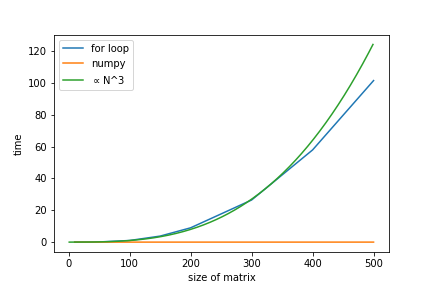
\includegraphics{p2.png}
    \caption{\textbf{P2: Matrix Multiplication} From the figure of operating time, we can see that as the size of the matrix $N$ increases, the operating time for for-loop method increases almost proportional to $N^3$, which is the number of operations it takes, while for numpy-dot method it stays the same. This suggests that np.dot() may be a more efficient method to do matrix multiplication when dealing with large matrices.
    }
    \label{fig}
\end{figure}

\section*{}

\begin{figure}
    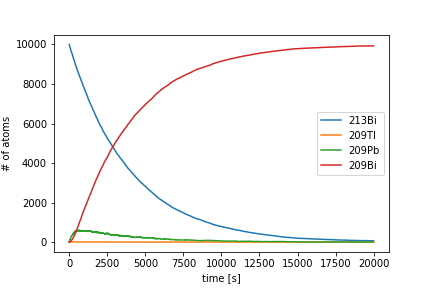
\includegraphics{p3.png}
    \caption{\textbf{P3: Decay Chain}
    Starting from 10000 213Bi atoms, we observe the decaying behavior of the four isotopes as shown. Notice that in each step, when deciding whether an atom decays or not will only change the number of the atom itself and the atom that it could decay into, thus we want to count from the bottom of the decay chain to top to avoid double counting.}
    \label{fig}
\end{figure}

\section*{}

\begin{figure}
    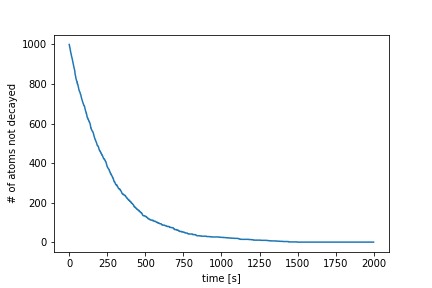
\includegraphics{p4.png}
    \caption{\textbf{P4: Decay by non-uniform distribution}
    Equation 10.5 gives the probability to decay at a certain time. Generating random numbers using this non-uniform distribution could give us a list of decay times. Then count the number of decay times that are later than the current time could give us the number of atoms that is not decayed at current time. To generate non-uniform distribution random numbers, we use Equation 10.10. I think this method could be more efficient if I could find the build-in function that could help me to count the number of elements in an array that is greater than a certain number.}
    \label{fig}
\end{figure}

\end{document}

 
 
